\chapter{Numerical analysis of spatial diversity}
\label{ch:numerical-simulator}
The previous chapter introduced the idea of exploiting spatial-diversity to provide more priority levels for flow classification. It was discussed why in principle such technique could yield flow completion time gains, especially when few priority queues are available. It was explained that adopting a spatial-diversity demotion has strong implication on the traffic load balancing, since flow routing becomes priority-dependent.  A few questions arises soon: how to choose the thresholds to distribute the load on the topology? What are the relationships between the priority granularity in 
single interfaces and spatial diversity? How to scale spatial diversity with the topology size? The goal of this chapter is to validate our intuitive hints with numerical results and to shed the light on the benefits and the restraints of the proposed algorithm. In particular, it will go through an exhaustive analysis of the system by delivering plenty of numerical experiments obtained with a custom flow level simulator implemented in Python. This simulator does not capture any of the complex dynamics inherent to a real packet network, it does not have any protocol stack implemented neither at traffic sources nor in the switching modules. Rather, it is a job-oriented queuing simulator that disregards packet level events but only runs flow arrivals and serve them in generic queues. Its purpose is to provide a clean baseline numerical analysis not plagued by possible side effects due to network misconfiguration.
Next sections will be an in-depth analysis of dynamics of the spatial diversity, when varying the dimensionality of the system both in the number of servers and in the number of priorities.
\section{Model implementation}

\subsection{Workloads}
\label{sec:workloads}
The performances of the three systems are compared using two empirical flow size distributions that have been derived from production data centers (Figure \ref{fig:workloads}). Flow size distribution is shortly termed \emph{workload}. The first workload has been estimated instrumenting thousands of servers in a datacenter hosting a Web search \cite{dctcp} application, while the other refers to data mining tasks \cite{vl2}. 
\begin{figure}
	\centering
	\begin{subfigure}[b]{0.49\textwidth}
		\centering
		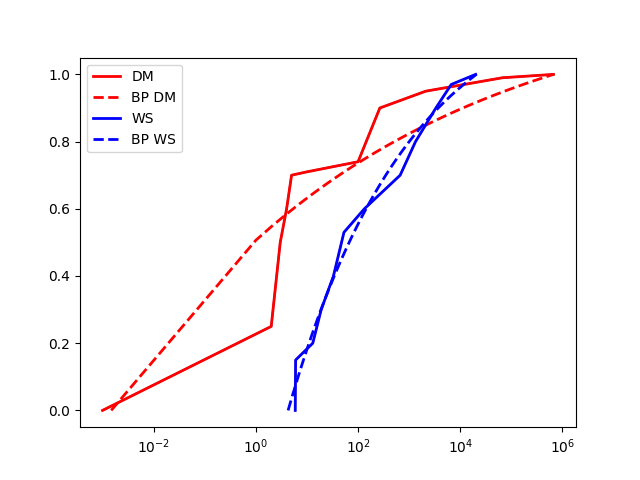
\includegraphics[width=\textwidth]{Chapter3/Figures/fits}
		\caption{CDF}
		\label{fig:cdfs}
	\end{subfigure}
   \hfill
   \begin{subfigure}[b]{0.49\textwidth}
   	\centering
   	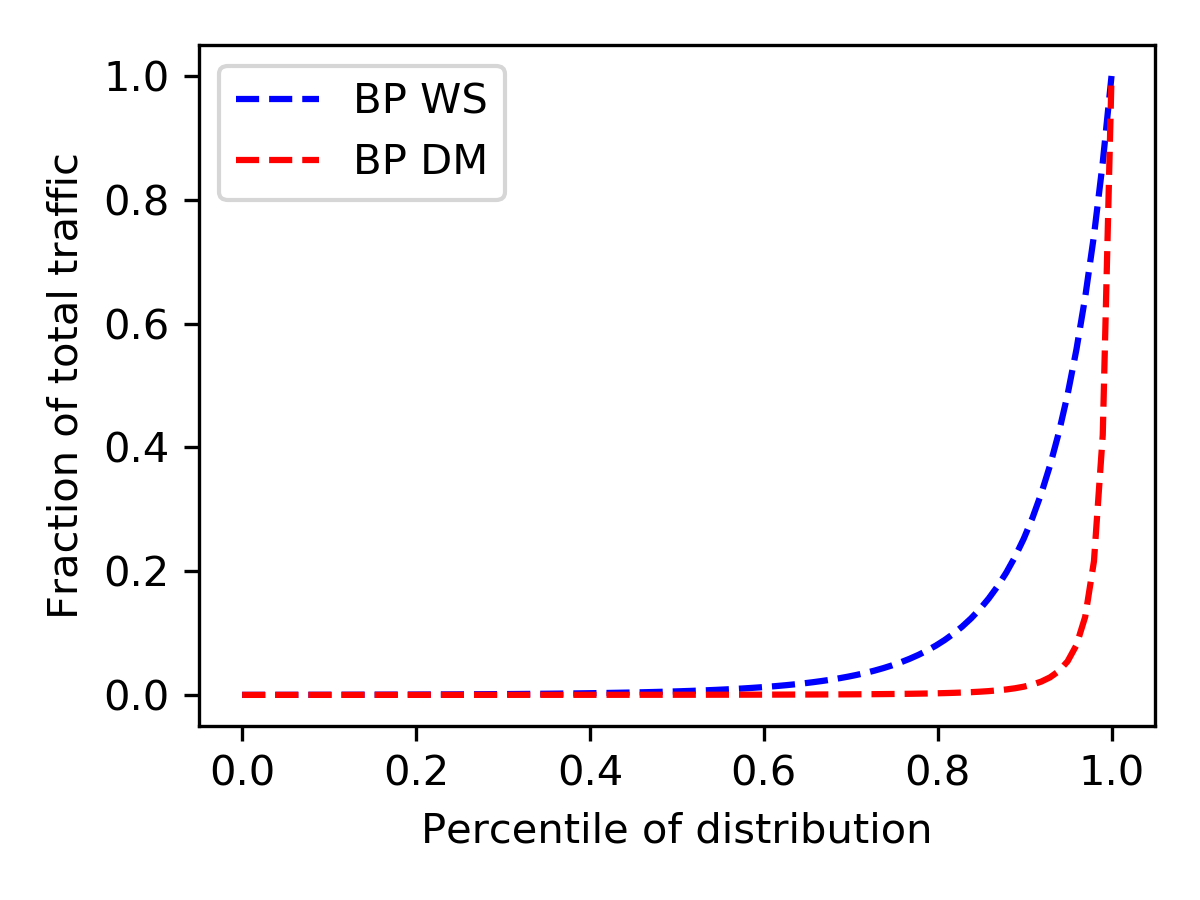
\includegraphics[width=\textwidth]{Chapter3/Figures/mwf}
   	\caption{MWF}
   	\label{fig:mwf}
   \end{subfigure}
	\caption{Workload properties}
	\label{fig:workloads}
\end{figure}
As expected, these distributions have a mix of short and long flows and both present the high-variability property typical of data center traffic (\S \ref{sec:traffic-properties}). Figure \ref{fig:cdfs} shows with solid lines the cumulative density function of the two empirical workloads, along with two analytical bounded Pareto distributions (dashed lines), whose parameters have been fitted to the corresponding empirical points. The bounded Pareto distribution is a truncated version of the Pareto distribution over the finite support $[u,t]$ and it is well-suited to model heavy-tail characteristics. It has three parameter: the lower extreme of its support $u$, the upper extreme $t$ and the shape parameter $\alpha$ that controls the weight of its tail. The analytical expression of its cdf $F(x)$ in the interval $[u,t]$ is:
\begin{equation}
	\label{eq:bpcdf}
	F(x) = \dfrac{1-\Big(\dfrac{u}{x}\Big)^{\alpha}}{1-\Big(\dfrac{u}{t}\Big)^{\alpha}}, \qquad 0 \le \alpha \le 2
\end{equation}
This distribution has been chosen to be used in the analysis due to some graceful properties. First of all, it is relatively easy to control its variability by a proper tuning of its parameter $\alpha$. Values of $\alpha$ close to 2 accentuate the heavy-tail property, while smaller values of $\alpha$ tend to regularize a bit its behavior. Second, being definite on a limited support it can be adapted to any minimum and maximum flow size in the datacenter. Third, the Pareto distribution is scale-invariant, meaning that normalized Pareto distributions remains Pareto. Nicely, this implies that the workloads observed by subsequent servers can be always modeled with the same probability distribution, only changing parameters. After all --- as seen in chapter \ref{ch:sdframework} --- these workloads  are conditional distribution obtained with simple normalizations. Last, its mean and its variance  --- which depend on $\alpha$ --- are finite, thus the problem of finding the shape parameter for any fixed first and second moment can be smoothly treated numerically. Specifically, for the bounded Pareto, the mean and the variance have the following expression:
\begin{align*}
\mathbb{E}[X] &= \dfrac{\alpha}{(1-\alpha)(t^{\alpha}-u^{\alpha})} (u^{\alpha}t - t^{\alpha}u) \\ \\
\sigma_X^2 &= \dfrac{\alpha}{(2-\alpha)(t^{\alpha}-u^{\alpha})} (u^{\alpha}t^2 - t^{\alpha}u^2)
\end{align*}
The best fit to the empirical distributions has been obtained with a simple Maximum Likelihood Estimator (MLE). The resulting parameters are reported for both the workloads. Let $X$ be the flow size random variable as usual, and write in short notation \textit{BP}($u,t,\alpha$) the bounded Pareto. 
\begin{align*}
	X_{WS} \sim& \text{\textit{BP}}(3, \, 29000, \, 0.125)\\
	X_{DM} \sim& \text{\textit{BP}}(0.1, \, 100000, \,0.26)
\end{align*}
The measurement unit for the extremes of the support in this case is kilobytes. The fitting error is higher for the data mining workload than for the web search. For low percentiles this is difficult to avoid because a very crude sampling is provided. In fact, on a total of 11 empirical points, 4 of them are for values above the 90th percentile. Instead, for high percentiles a better fitting likely could be obtained by weighting more the tail of the distribution. \\
The rightmost plot (Fig. \ref{fig:mwf}) completes the picture by showing the Mass-Weighted Function $M_w(x)$ \cite{mwf}. This can be seen as the probability that a byte picked at random belongs to a flow below a given percentile and it is used to characterize the variability of a distribution. Its name comes from its definition, where job sizes are weighted by their probability mass:
\[
M_w(x) = \dfrac{\int_{0}^{x} x f(x) dx}{\mathbb{E}[X]}
\]
It holds:
\[
\int\nolimits_{0}^{x} x f(x) dx \le \mathbb{E}[X]
\]
In other words, it is just the average normalized traffic injected by flows shorter than $x$. The figure has on the abscissa the percentile rather than the corresponding job size, to allow the comparison between workloads with different supports on the same axis. If $y$ is a given percentile, it is evaluated $M_w(F^{-1}(y))$. \\
In summary, both distributions exhibit high variability. In the web search case the largest 4\% of flows carry half of the total traffic, the data mining is even more skewed: 70\% of the flows are less than 8 packets only, but almost the entire load is sustained by a ridiculous percentage of flows of about 100MB of size. This suggests that the more challenging distribution to schedule is the web search, consequently it is the one that will deserve most of the attention. In fact, recall that an ideal flow-agnostic LAS scheduler guarantees lower and lower delays as the variability of the distribution increases, both on average and at high percentiles (\S \ref{sec:las}). The theory is confirmed pretty straightforwardly by the simulation results presented next. Moreover, the web search distribution is also a lot easier to simulate, since the very long tails of the data mining workload require protracted time-consuming simulations before being precisely reproduced. Long flows occur sporadically, however they give the main contribution to generate a desired load on the system. 

\subsection{Optimal traffic load balancing}
In previous discussions, it was already realized that the spatial diversity framework introduces strong implications on how the load is distributed on the switching fabric. We decided to solve an optimization problem with the goal of finding the optimal load balancing and then to treat sub-thresholds a posteriori (\S \ref{sec:decoupling}). Thus, we considered the abstraction of spatial diversity as a queuing system (\S \ref{sec:threesystemcomparison}) setting $N$=1 priority queue per server. With this setup all flow demotions correspond to shifting a flow from one server to the other. This way, the original problem of jointly optimizing inter and intra server demotion at once, has been simplified to finding the load balance that minimize the average flow completion time. \\
In this section we first start by analyze the simpler example of spatial diversity, where only two M/M/1 servers are deployed in parallel, each of them with only a single priority queue. In this case there is globally only one threshold, therefore it's possible to plot the shape of the cost function and to study its properties. It is worth remarking again that this threshold is a load balance threshold, therefore the following analysis will refer to the load balancing minimization problem, where there isn't any strict priority scheduler and all servers work in parallel with full capacity $\mu/K$. In other words, there is not any throttling that would assign only the residual capacity to the low priority server (already discussed in \S \ref{sec:decoupling}).  We start initially by solving the formulation for M/M/1 queues, then we will look for the solution of M/G/1 as well. For the sake of simplicity, we have implemented a total service rate $\mu = \mathbb{E}[X]$. In this way the average load fed in the system 
\[
\rho = \frac{\lambda}{\mu}\;\mathbb{E}[X]
\]
is given only by the flow arrival intensity $\lambda$.

\begin{figure}
	\centering
	\begin{subfigure}{.5\textwidth}
		\centering
		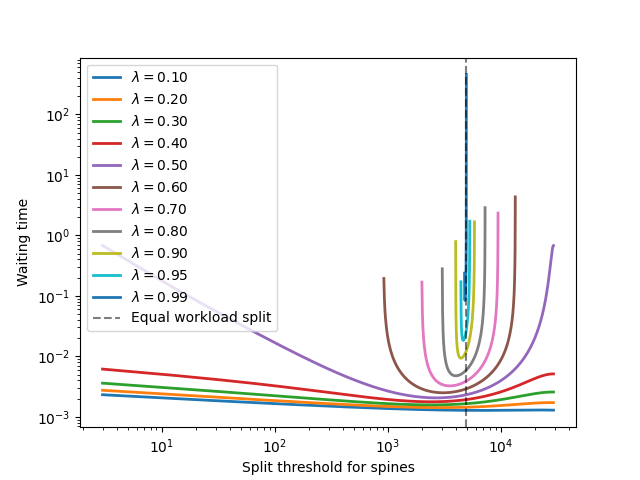
\includegraphics[width=.99\linewidth]{Chapter3/Figures/equal_workload_split_bpws}
		\caption{Optimal load balance threshold}
		\label{fig:cost-ws}
	\end{subfigure}%
	\begin{subfigure}{.5\textwidth}
		\centering
		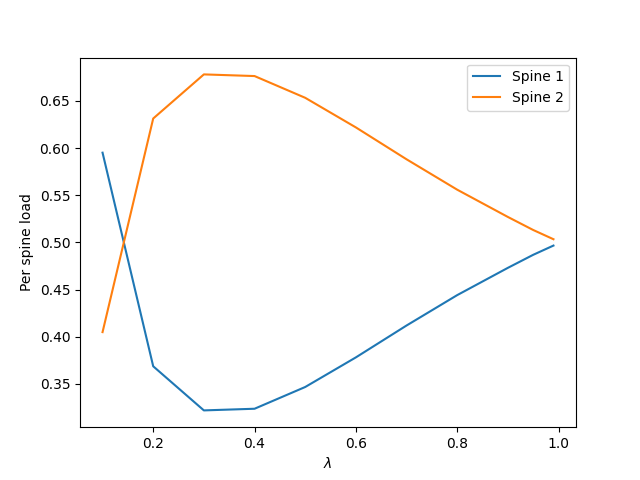
\includegraphics[width=.99\linewidth]{Chapter3/Figures/per_spine_load_bpws}
		\caption{Load distribution per-server }
		\label{fig:perspineload-ws}
	\end{subfigure}
	\caption{Web search workload. Simple case of $K$=2.}
	\label{fig:lbthreshold-ws}
\end{figure}

\begin{figure}
	\centering
	\begin{subfigure}{.5\textwidth}
		\centering
		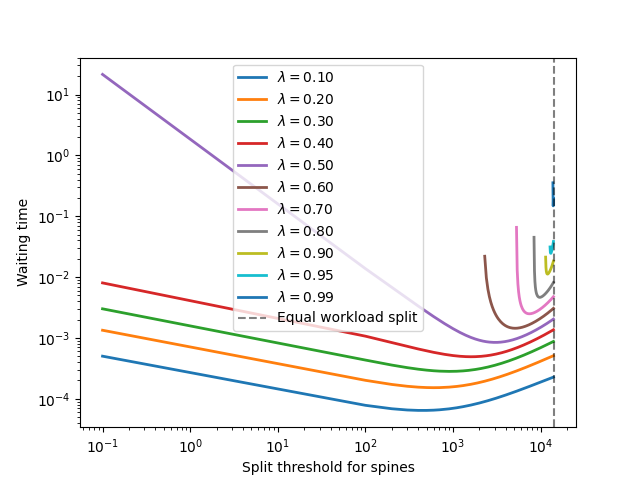
\includegraphics[width=.99\linewidth]{Chapter3/Figures/equal_workload_split_bpdm}
		\caption{Optimal load balance threshold}
		\label{fig:cost-dm}
	\end{subfigure}%
	\begin{subfigure}{.5\textwidth}
		\centering
		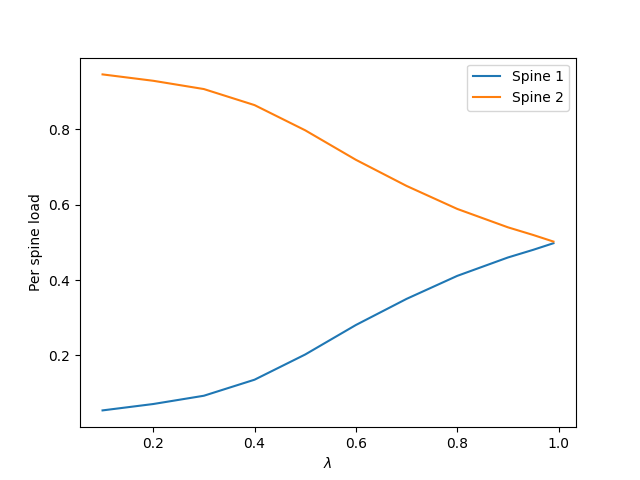
\includegraphics[width=.99\linewidth]{Chapter3/Figures/per_spine_load_bpdm}
		\caption{Load distribution per-server }
		\label{fig:perspineload-dm}
	\end{subfigure}
	\caption{Data mining workload. Simple case of $K$=2.}
	\label{fig:lbthreshold-dm}
\end{figure}%TODO per spine load measured or plugged threshold in equation? 
\subsubsection{Load balance on 2 parallel servers}
\label{sec:load-balance-2-servers}
In the basic case of $K$=2 parallel servers, it is possible to plot the average sojourn time when varying the load balance threshold. Figures \ref{fig:cost-ws} and \ref{fig:cost-dm} show how the cost functions look like, for the web search and the data mining workloads, respectively. All the axes are in log-scale and each curve represents a different normalized traffic $\lambda$. The vertical lines correspond to the split that gives perfect load balance, apportioning half of the traffic on the high priority server and half on the low priority one. This split may be interchangeably referred to as \emph{perfect split} or \emph{proportionate split} in the following. Figures \ref{fig:perspineload-ws}-\ref{fig:perspineload-dm} show in parallel the normalized traffic distribution on the two servers, corresponding to the optimal threshold. One phenomena is visible for both workloads, confirming previous intuitions. The optimal load balance threshold does not coincide, broadly speaking, with the proportionate split threshold. Depending on the traffic level at which the system is operated and the workload, the optimal threshold triggers an earlier or later demotion with respect to the perfect split case. Equivalently, the jobs are distributed unfairly between the two servers (Figures \ref{fig:perspineload-ws}-\ref{fig:perspineload-dm}). Imagine to connect the absolute minimums of the cost functions. For data mining, the imaginary line would be always in the leftmost side with respect to the proportionate split. That is, apart from loads close to saturation, the high priority server is kept as jobless as possible and the majority of work is sent to the low priority server. Remember that the problem formulation weighted the average sojourn times in the $i$-th priority queue with the percentage of flows with size between the thresholds $\alpha_{i}$ and $\alpha_{i+1}$. The objective was:
\[
\mathcal{T} = \sum_{i=1}^{N}\textcolor{red}{\theta_i} \sum_{j=i}^{N}T_j
\]
Since the data mining workload is highly dominated by short flows, they receive more importance and longer flows are moved soon to another path. Plenty of short flows carrying few bytes are kept on a separated link from medium sized flows and a couple of long flows. Thus, the result is not a surprise but it is coherent with the flow distribution. \\
Slightly different trend is observed for web search. Moving from low to high values of $\lambda$, the optimal threshold is initially greater than the perfect split axis, then switches to its left and finally the two coincide. This is clear from the load distribution on the two servers. In general, for web search the load remains more balanced between the two servers in respect to data mining. The more unbalanced split occurs at $\lambda$=0.3 where 70\% of the traffic is handled by the low priority server. Instead, data mining has much more extreme load subdivision, especially for $\lambda$=0.1. This is a consequence of the high variability of the workload: there is six order of magnitude difference between the shortest and the longest flow and there is a pronounced heavy-tail. Hence in order to have significant changes on the weights $\theta_i$ the threshold is moved significantly along the heavy-tail. In other words, the optimal threshold reroute few flows but lot of traffic on the low priority server. In fact, for $\lambda$=0.1 the absolute value of the optimal threshold is much smaller than the proportionate split threshold, however only a small fraction of flows fits into this gap. Also, for similar reasoning, the two workloads have different sensitivities to the load balance threshold optimization. In particular, the web search achieves appreciable FCT gains starting from medium loads only ($\lambda > 0.5$) with a factor 2 gain%\textcolor{red}{(TODO provide some numbers)}, 
whereas at low loads there is no practical difference with the proportionate split. On the contrary, the data mining distribution gives theoretically an order of magnitude %\textcolor{red}{(TODO provide some numbers)} 
lower waiting time even for $\lambda$=0.1. %This again reflects the extreme variability of the workload, that is comprised by a disproportionate number of short flows. %The perfect split would keep a lot of mice flows mixed with low priority flows of bigger size for protracted service time. Instead, 
Finally, for both cases the objective function becomes much more extremely curled and steep around the perfect split axis when the load approaches the saturation value 1.  As already remarked, this is inevitable in order to fully exploit all the available capacity offered by the two parallel servers. At so high load any other traffic split would overload one of the two links and strongly deteriorate the average completion time of the flows going through it. Consistently, the cost function grows very rapidly in the neighborhood of the perfect split threshold value. Indeed, the M/M/1 response time $T$ grows exponentially close to saturation. Its law (Figure \ref{fig:mm1-responsetime}) is:
\[
T \propto \dfrac{1}{1-\rho}
\]
\begin{figure}
	\centering
	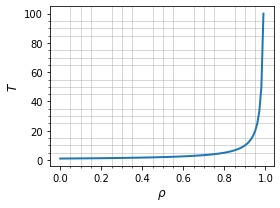
\includegraphics[width=0.4\textwidth]{ChapterSpatialDiversityFramework/Figures/mm1-response-time}
	\caption{M/M/1 response time}
	\label{fig:mm1-responsetime}
\end{figure}
\subsubsection{Validity of the optimal load balance model}
Summarizing, the above discussion confirms that the web search traffic is harder than the data mining to cope with. This is the reason why in the following some results are shown exclusively for this workload. 
Next, it is consolidated the validity of the stochastic optimization model with numerical flow level simulations, in particular it is shown the effective benefit of optimal load balancing. The underlying topology is again the simplest one, comprised of two parallel M/M/1 servers with no inner prioritization. The serving discipline is Processor Sharing (PS), implemented with a fluid model where parallel flows are served with equally subdivided bandwidth. 
The average normalized flow completion time (nFCT) has been considered as the primary evaluation metric.
\smallskip
\begin{tcolorbox}[title=Definition]
	\textbf{nFCT}: Given a fixed data center topology and pair of source-destination servers, \{$s$, $d$\}, define $FCT_{opt}(x)$ as the FCT achieved by a flow of length $x$ originated from $s$ and directed to $d$ in a completely empty DCN at load zero (excluding such a flow). Let $FCT(x)$ be the FCT of a flow of length $x$ in a DCN in the presence of other flows. Let $X$ be the set of all possible flow lengths. Define:
	\[
	nFCT = \sum_{x \in X} \small \frac{FCT(x)}{FCT_{opt}(x)} \normalsize.
	\]
\end{tcolorbox}
\smallskip
The normalized flow completion time is very similar in spirit to the average slowdown presented in Sec.\ref{sec:las}, but it is more handful as it is dimensionless. Its advantage is to put all flows on the same comparable scale, permitting a clean visual analysis of fairness with respect to flow size. By the way, this kind of evaluation is important to us, as spatial diversity mainly targets short and medium flows by augmenting the priority granularity. \\
Figures \ref{fig:optlb-ws}-\ref{fig:optlb-dm} report the nFCT gain obtained thanks to the sole load balance optimizer. 
\begin{figure}
	\centering
	\begin{subfigure}{.5\textwidth}
		\centering
		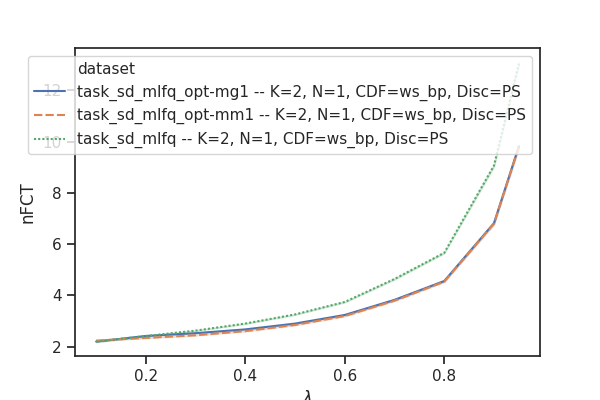
\includegraphics[width=1.05\textwidth]{Chapter3/Figures/ws_ps_comparison}
		\caption{nFCT comparison}
		\label{fig:optlbgain-ws}
	\end{subfigure}%
	\begin{subfigure}{.5\textwidth}
		\centering
		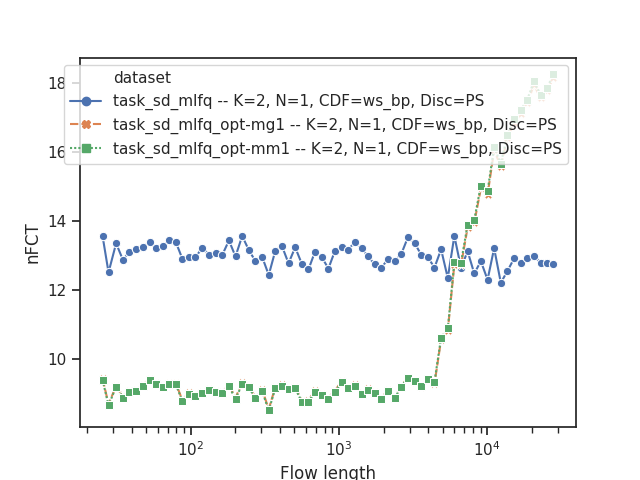
\includegraphics[width=\textwidth]{Chapter3/Figures/ws_ps_detailed.png}
		\caption{Per-flow length nFCT. $\lambda=$0.9}
		\label{fig:optlbgainvsflowsize-ws}
	\end{subfigure}%
	\caption{Web Search workload}
	\label{fig:optlb-ws}
\end{figure}%
\begin{figure}
	\centering
	\begin{subfigure}{.5\textwidth}
		\centering
		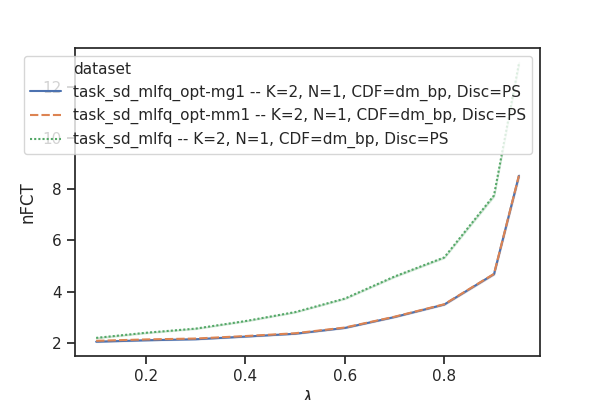
\includegraphics[width=1.05\textwidth]{Chapter3/Figures/dm_ps_comparison.png}
		\caption{nFCT comparison.}
		\label{fig:optlbgain-dm}
	\end{subfigure}%
	\begin{subfigure}{.5\textwidth}
		\centering
		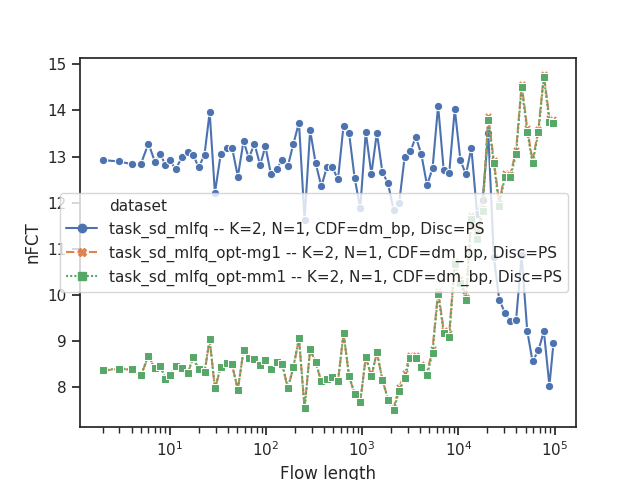
\includegraphics[width=\textwidth]{Chapter3/Figures/dm_ps_detailed.png}
		\caption{Per-flow length nFCT. $\lambda=$0.9}
		\label{fig:optlbgainvsflowsize-dm}
	\end{subfigure}%
	\caption{Data Mining workload}
	\label{fig:optlb-dm}
\end{figure}%
Two different scenarios are compared. Both adopt spatially-diverse MLFQ, but in one case the load balance threshold is optimized, in the other not. The former case is labeled as \texttt{SD-MLFQ-OPT}, whereas the latter as \texttt{SD-MLFQ}. Call $s_0$ and $s_1$ the two servers (i.e links/queues) and $\Omega$ the unique demotion threshold. Newly arrived flows always enter the system through $s_0$ as their attained service equals to 0, then they are rerouted to the link $s_1$ when server $s_0$ has transmitted $\Omega$ of their bytes. As expected, the benefits on the average completion times are more pronounced for the data mining distribution, at all loads (Figures \ref{fig:optlbgain-ws}-\ref{fig:optlbgain-dm}). Even so, appealing phenomena emerge when looking at the detailed breakdown of the response time versus flow size (Fig.\ref{fig:optlbgainvsflowsize-ws}-\ref{fig:optlbgainvsflowsize-dm}). First focus on the SD-MLFQ system without load balancing optimization and compare the blue curves. In web search, the normalized response time curve exhibits a constant plateau which testify a substantial invariance of the slowdown with respect to the flow length. Conversely, in data mining there is an abrupt transition to lower response times for flows longer than 20MB, which roughly corresponds to the demotion threshold adopted in this case. The difference is justified by the fact that the proportionate split threshold for data mining cuts the flow size CDF near the 99-th percentile, due to the oft-repeated heavy-tail characteristic of this workload. Therefore, only few long flows remain to share the processor of the low-priority server $s_1$.  Since the  nFCT captures the slowdown in respect to the ideal case where the flow is serviced alone, it is reduced when less flows contend the bandwidth. This is true as long as PS all servers use the PS discipline. \\
Next, let's concentrate on the spatial diversity with optimal load balancing (green curves), which is the real experiment needed in order to validate the model. The two workload perform similarly and have analogous trends. More importantly, the encouraging result is that short and medium flows indeed take advantage of spatial diversity, as they are sent through a less loaded path. For the data mining case, there is approximatively a 35\% gain for flows smaller than 6MB. The opposite happens to long jobs, which undergone the dual effect.
% TODO definition of main spatial diversity principles (bullet item list)
% TODO M/M/1 vs M/G/1 how implemented in practise? Assumed poisson arrivals but not true....what changed? How determined the variance of the job for subsequent servers? 
\subsubsection{Finding optimal load balance with Basin-hopping}
So far the only scenario that has been investigated is the simple case of two parallel servers without sub-thresholds. This was useful to get confident with the relationships between load balance and the spatial diversity demotion mechanism. However, in the more general setting there might be much more parallel servers and at least two priority levels per server. The total number of thresholds was reduced by decoupling the load distribution by the server-local prioritization. Thus, the total complexity only depends on the number of servers $K$. Unfortunately, it is still typically high. 
%\textcolor{red}{TODO basin hoppin brief description (GERMAN) + parameter setting of the solver (GERMAN) + solution time plot descrioption (ALE)}
Basin-hopping is a meta-heuristic which provides means of solving non-convex optimization problems.
It operates on an iterative basis by selecting random starting point in possible solution state-space and performing local minimization. 
Subsequently the process is repeated by "hopping" to a different point and re-performing minimum search.
We consider BFGS as a local minimization algorithm, we set a step size equals to 100 for random perturbation as it was empirically found to be a good trade-off between convergence speed and accuracy.
We then perform 300 iterations for each point in \textbf{figura con i load} on a Intel i7-7700k with 16GB of RAM.
% dire python scipy solver
% TODO citare basin hoppin e pso heuristics (some parameters used, bla bla)
% TODO why complexity is higher at load 0.6 ???
\section{Dimensioning spatial diversity}
In the previous section it was laid down the basic framework of spatial diversity. It was remarked the fact that adopting spatial diversity translates into a priority-driven load balancing. At the same time were collected encouraging results about the effectiveness of the optimal load balancing. It was discussed the impact of two workloads commonly used as a benchmark in literature. Then, it was solved the optimal load balancing problem for up to $K$=9 parallel servers ans shown that for large topologies we may incur in overwhelming complexity. In all the simple experiments carried out, the servers were always configured with Processor Sharing service discipline and without priority queues.

This section aims to provide answers to principally two things. The first one is the behavior of the priority-driven load balancing when increasing the number of server $K$ up to 9 parallel servers. Thus, we try to evaluate the effects of the load balance thresholds alone with bigger topologies, initially disregarding sub-thresholds again. Second, it is treated the integration of the priority-driven load balancing with the legacy MLFQ system. In practice, it is considered the general case where each server has many PQs on its interfaces used in strict priority. As it will be explained shortly, it turns out that for both attempts, the performances of the system are highly correlated with the adopted servicing policy. The two considered cases are the FIFO (FCFS) servers and the usual PS servers. 

\subsection{Effects of SD-rank and PQ granularity}
\label{sec:dimensioning-spatial}
First it is addressed the first question: what are the effects of augmenting the spatial diversity \emph{rank}? 
\begin{tcolorbox}[title=Terminology]
	\textbf{SD-rank}: Given a data center topology with $S$ spines --- or the equivalent system of parallel M/M/1 servers where is applied priority-driven load balancing, that is each server handle a group of priority and a flow is routed depending on its assigned priority. Let's define the spatial-diversity rank (SD-rank) as the number $K$ of servers which handle different priorities. 
\end{tcolorbox}
The spatial diversity ranks tells how many M/M/1 servers (or group of servers) are considered to be used to implement spatial diversity. For example, suppose there are 4 parallel servers available $s_0$, $s_1$, $s_2$, $s_3$. Consider these two possibilities. 
\begin{enumerate}
	\item \textbf{Rank 2}. The four servers are grouped in two pairs, say $(s_0, s_1), (s_2,s_3)$. Spatial diversity demotion is applied at pair level. This means there is only one load balance threshold $\Omega$. When the longest flow enters the system, it is sent at random either on $s_0$ or $s_1$. As soon as the flow has received service $\Omega$ it is demoted, again randomly, either on $s_3$ or $s_4$. In other words, this can be seen as a system of only two parallel servers with twice the capacity each, where only one rerouting happens to the longest flow. 
	\item \textbf{Rank 4 \textit{(full-rank)}}. The servers are not grouped in any way. All servers participate to the priority-driven load balance. Therefore, there are 3 thresholds and the longest flow it is rerouted three times.
\end{enumerate}
In the next experiments (Fig.\ref{fig:lb-var-K-fifo}) is evaluated the full-rank spatial diversity system for three topologies, corresponding to $K=3$, $K=5$, $K=9$ and for two serving policies: PS and FIFO. The number of priority queues $N$ is still one per server. Remember that the numerical simulator is a job level simulator, thus flows are not fragmented in packets anyhow. This means that the FIFO policy is absolutely non-preemptive for jobs in the same priority queue. The service of a flow cannot be interrupted and flows arriving in the meanwhile are queued back in a first-in first-out order. Instead, the PS discipline subdivides the available capacity among all flows present in the system with a fluid approximation. Thus, a fresh flow share immediately the service rate granted to its priority queue with other flows in the same queue. 
\begin{figure}
	\centering
	\begin{subfigure}{.5\textwidth}
		\centering
		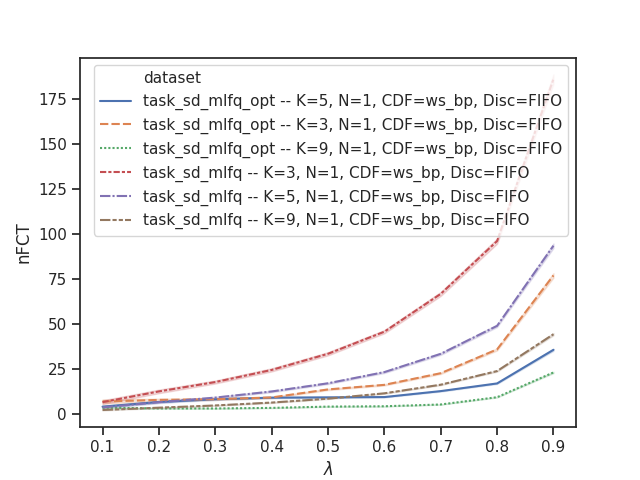
\includegraphics[width=0.99\textwidth]{Chapter3/Figures/lb_opt_vs_nopt_comparison}
		\caption{nFCT comparison}
	\end{subfigure}%
	\hfill
	\begin{subfigure}{.5\textwidth}
		\centering
		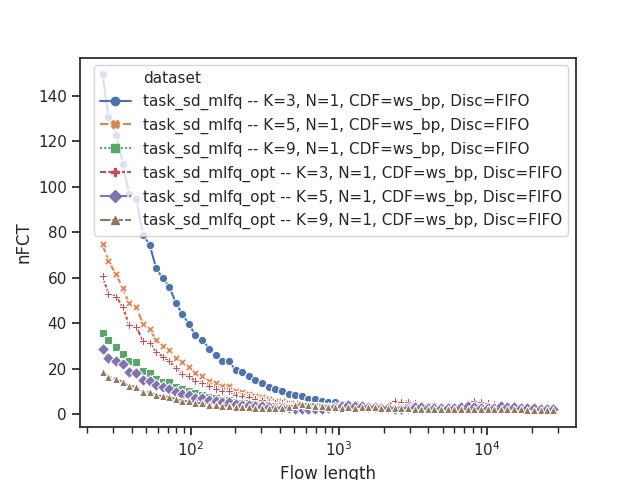
\includegraphics[width=0.99\textwidth]{Chapter3/Figures/lb_opt_vs_nopt_detailed}
		\caption{Per-flow length nFCT ($\lambda$=0.9)}
		\label{fig:lb-var-K-fifo-detailed}
	\end{subfigure}
	\caption{Web Search workload and FIFO discipline at 99\% confidence interval.}
	\label{fig:lb-var-K-fifo}
\end{figure}
\begin{figure}
	\centering
	\begin{subfigure}{.5\textwidth}
		\centering
		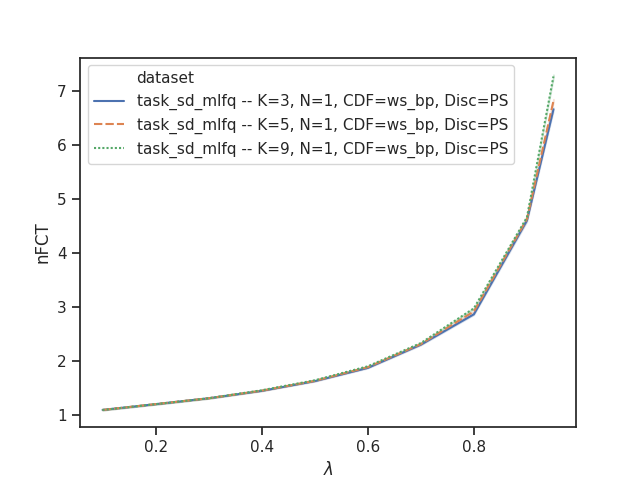
\includegraphics[width=0.99\textwidth]{Chapter3/Figures/lb_opt_vs_nopt_comparison_fifo}
		\caption{nFCT comparison}
	\end{subfigure}%
	\hfill
	\begin{subfigure}{.5\textwidth}
		\centering
		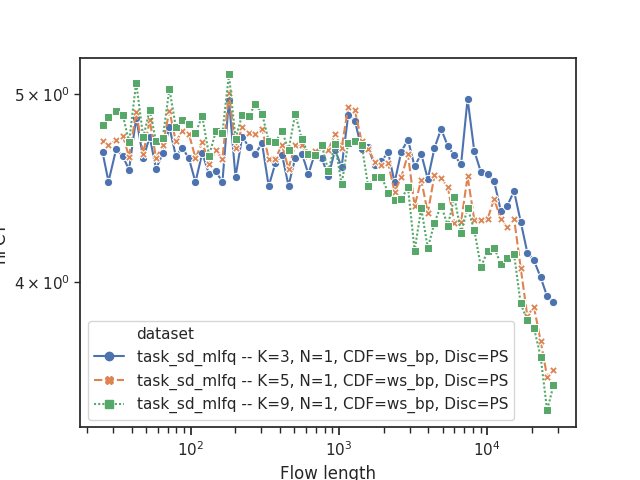
\includegraphics[width=0.99\textwidth]{Chapter3/Figures/lb_opt_vs_nopt_detailed_ps}
		\caption{Per-flow length nFCT ($\lambda$=0.9)}
		\label{fig:lb-var-K-ps-detailed}
	\end{subfigure}
	\caption{Web Search workload and PS discipline at 99\% confidence interval.}
	\label{fig:lb-var-K-ps}
\end{figure}
%TODO when N=2 and FIFO what's the policy?
These experiments were carried out both with and without the optimized load balance thresholds. Whenever load balance thresholds are not optimized, it is used the proportionate split criterion. Experiment are shown for the web search workload only, which is the more challenging to handle. The first very positive observation is that, whatever the number of servers, the optimal load balance wins over the proportionate split. This again confirms the validity of the queuing model formulation for load balancing. 
The FIFO policy is clearly unfair with respect to short flows (Fig.\ref{fig:lb-var-K-fifo-detailed}). This is because without preemption a single elephant flow could starve a myriad of short flows. This does not happen with PS, because short flows always share the processor with other longer flows. Indeed, in absolute terms the PS discipline overcome of two order of magnitude FIFO, remarking the fact that under the assumption of high variability of the distribution, it is better to adopt a PS policy. The unfairness of FIFO is mitigated when increasing the spatial diversity rank, because long flows are demoted earlier and leave quickly high priority servers. Notably, for a fixed $K$, having $N$=1 priority queue is the worst case from the point of view of mice flow starvation. With $N$>1 PQs, the service received by a flow on each server would be broken in multiple phases, each on a different priority queue. Since the PQs are scheduled in Strict Priority order and newly arrived flows enter in high priority, a short flow behind longer ones would have to wait only until the demotion at lower priority of the flows ahead. Somehow the demotion preempts the long flows, and weaken the impact of having a FIFO policy on the PQs themselves. \\
Not surprisingly, when increasing the rank there is not a significant change in the average flow completion time with PS. In the web search distribution a relevant role is played by medium flows. Thus, increasing the number of inter-server demotions without any intra-server demotion hasn't any effect on FCT minimization. Medium flows stay anyway with elephant flows, only across more parallel servers. This clearly indicates that the priority dependent load balance alone is not enough with PS. On the other hand, for higher rank we start observing on elephant flows the same trend that was observed in Fig.\ref{fig:optlbgainvsflowsize-dm} for the data mining workload but not for the web search. In that section, (\S \ref{sec:load-balance-2-servers}) we had only 2 parallel servers and we argued that this gain for the elephant flows happened because only few simultaneous flows shared the processor of the lower priority server. Here the same happens also for the web search distribution, since there are enough demotions to truncate the distribution at high percentiles and leave few flows for low priority servers.

The study of the system with increased number of priority queues led to even more surprising results. This step really integrates the spatial diversity in the legacy MLFQ system with many priority levels. Here it is reported only the Processor Sharing discipline for the reasons explained few lines above: it is clear that for FIFO increasing $N$ would further reduce the average flow completion time. A numerical proof confirming this fact (Fig. Fig. \ref{fig:esn-vs-sdmlfq-fifo-fixed-K}) will be shown in the last section \S \ref{sec:final-comparison} of the chapter during the final comparisons of SD-MLFQ with ES-N. \\
Figure \ref{fig:sdmlfq-variable-N} is a key result that will uncover potential bottlenecks of SD-MLFQ. In this experiments are compared the average flow completion times of the system with fixed $K$=4 and variable $N$. Load balance thresholds are not optimized in this case, but are set to grant the proportionate split of the traffic on the four parallel servers. The sub-thresholds have been assigned with the simple ES-N variation for spatial diversity (\S \ref{sec:subthresh-with-sd}). Very interestingly, this numerical results provide a different perspective on the best granularity of priority queues per server when introducing spatial diversity. While on the systems that approximate LAS or SRPT schedulers \cite{pias, pFabric}, increasing the number of priority queues is always beneficial, it is not so when spatial diversity is adopted. At low load there is not a visible difference among the simulated scenarios. However, at high load the best average nFCT is attained with $N$=2 priorities per server (dashed orange curve). The peculiar phenomenon is the behavior of the case $N$=8 (red curve), whose corresponding nFCT starts to increase consistently above $\lambda=0.8$. 
\begin{figure}
	\centering
	\begin{subfigure}{.5\textwidth}
		\centering
		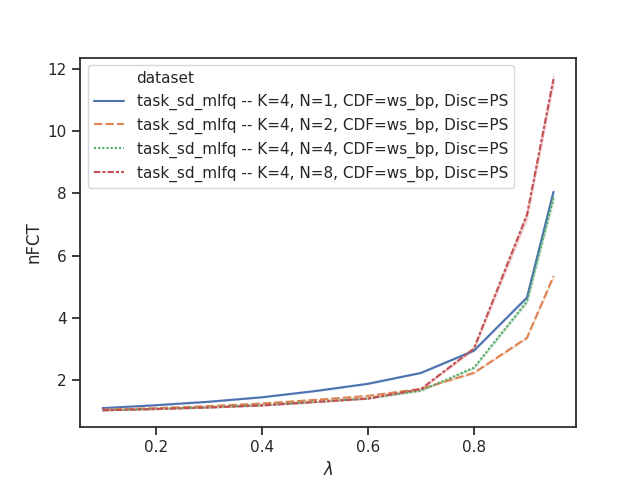
\includegraphics[width=0.99\textwidth]{Chapter3/Figures/sd_mlfq_k4_comparison.png}
		\caption{nFCT comparison}
		\label{fig:sdmlfq-variable-N-fct}
	\end{subfigure}%
	\hfill
	\begin{subfigure}{.5\textwidth}
		\centering
		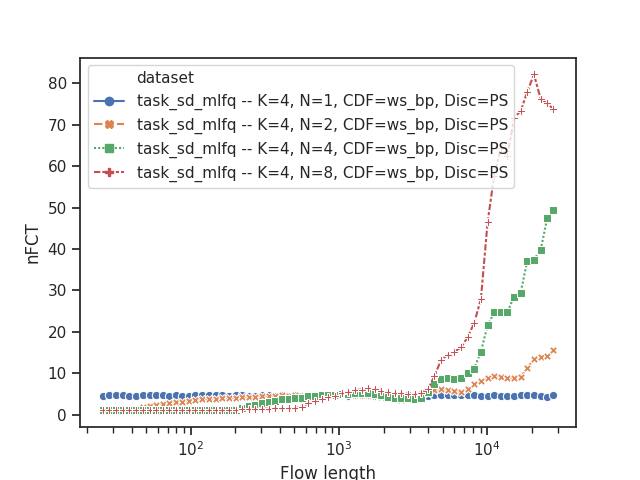
\includegraphics[width=0.99\textwidth]{Chapter3/Figures/sd_mlfq_k4_detailed.png}
		\caption{Per-flow length nFCT ($\lambda$=0.9)}
		\label{fig:sdmlfq-variable-N-fct-detailed}
	\end{subfigure}
	\caption{Effects of intra-server demotion with spatial diversity. Results shown for web search workload, PS and fixed $K=4$. Results plotted with 99\% confidence interval.}
	\label{fig:sdmlfq-variable-N}
\end{figure}
From the detailed breakdown of Fig.\ref{fig:sdmlfq-variable-N-fct-detailed}, it is evinced that the most severe degradation happens to long flows. As a general trend, an higher number of priorities per server is reflected in a more pronounced raise of the job response time of long flows. At the same time, coherently with the scheduling theory of LAS (\S \ref{sec:las}) and the results of PIAS, flows between 100KB and 1MB (medium size flows) are improved. However, long flows suffer an unacceptable penalty, which globally makes also the average worse.  \\
We repeated the same experiment with the smallest possible rank that guarantees the applicability of spatial diversity, that is $K$=2. The results are shown in Fig. \ref{fig:sdmlfq-variable-N-K2}. 
\begin{figure}
	\centering
	\begin{subfigure}{.5\textwidth}
		\centering
		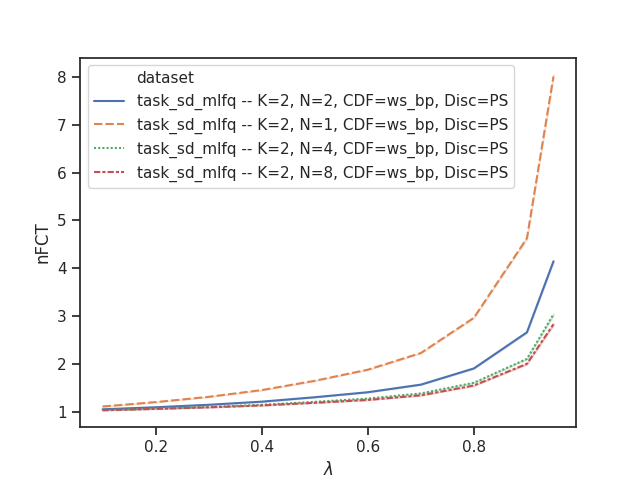
\includegraphics[width=0.99\textwidth]{Chapter3/Figures/sd_mlfq_k2_comparison.png}
		\caption{nFCT comparison}
		\label{fig:sdmlfq-variable-N-fct-K2}
	\end{subfigure}%
	\hfill
	\begin{subfigure}{.5\textwidth}
		\centering
		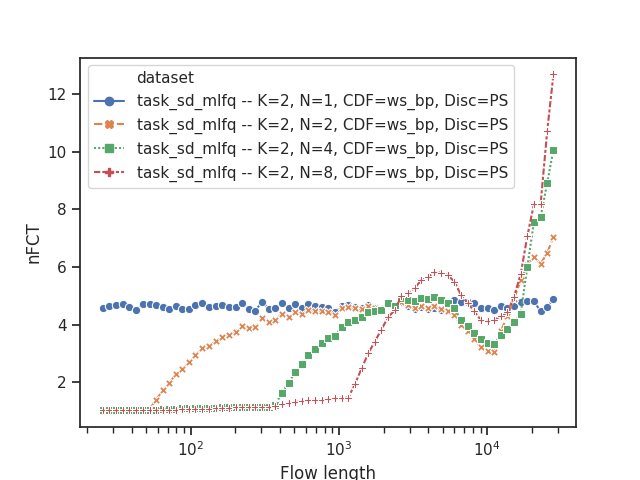
\includegraphics[width=0.99\textwidth]{Chapter3/Figures/sd_mlfq_k2_detailed.png}
		\caption{Per-flow length nFCT ($\lambda$=0.9)}
		\label{fig:sdmlfq-variable-N-fct-detailed-K2}
	\end{subfigure}%
	\caption{Effects of intra-server demotion with spatial diversity. Results shown for web search workload, PS and fixed $K=2$. Results plotted with 99\% confidence interval.}
	\label{fig:sdmlfq-variable-N-K2}
\end{figure}%
Intriguingly, the problem on longer flows starts to reveal, but with less intensity. This suggests some correlation between the spatial diversity rank and the critical behavior of long flows, especially when there are 8 priority queues per server.  Short and medium flows experience exactly the same trend as in the case $K$=4, but in this case it is visually more clear (Fig.\ref{fig:sdmlfq-variable-N-fct-detailed-K2}) because it is not squeezed by the scale of y-axis. 
\subsection{Impairments of spatial-diversity}
\label{sec:sd-impairments}
Summarizing, the previous experiments leave the following remarks as concerns the Processor Sharing (PS) discipline:
\begin{itemize}
	\item \textbf{Remark 1. \textit{Impact of PQ granularity}.} Whatever the spatial diversity rank (number of parallel servers across the which is applied spatial diversity), there is a nFCT penalty for long flows in using more than $N$=2 priority queues per server.
	\item \textbf{Remark 2. \textit{Impact of SD-rank}.} When $N>1$, that is when intra-server demotion is applied, increasing the spatial diversity rank rapidly exacerbates the nFCT impairments on long flows. The performance drop may become unacceptable and dominate the behavior of the average FCT curve.
\end{itemize}
Such an extreme behavior on long flows was worth of extra-attention. In particular, it brings up two important questions: why does it happen? Is the best choice to continue demotion also in low priority servers?
We concern why spatial diversity exacerbates the unfairness of the scheduler with respect to longer flows. The fact that long flows are penalized is not new. Both LAS, the theoretical scheduling policy, and MLFQ, its approximation with priority queues, suffered the problem of long flows starvation. Nonetheless, the spatial diversity presents a peculiar impairment that worsen the performances if the size of the topology --- precisely the SD-rank --- grows. We identified two causes of the problem: demotion in low priority servers and flow synchronization. Unfortunately, both of them are either originated or amplified by the spatial diversity. 
\subsubsection{Demotion in low priority servers}
We ask whether it is meaningful to exploit all available priority queues in low priority servers for flow demotion, or not. We addressed this problem by looking at the simple scenario of $K=N=2$ with the web search workload. This setting allows to have a single load balance threshold and a single sub-threshold in each server $s_1,s_2$. Then, we tried to optimize the sub-threshold on the low priority server, for any possible load balance threshold. This step was easily treatable numerically with a brute-force minimization, as there is only one sub-threshold.
\begin{figure}
	\centering
	\begin{subfigure}{.5\textwidth}
		\centering
		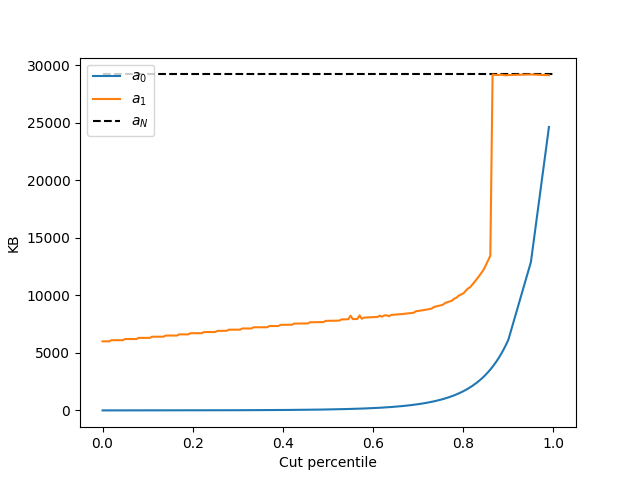
\includegraphics[width=0.99\textwidth]{Chapter3/Figures/cut_demotion}
		\caption{Optimal sub threshold for $s_2$ ($\lambda=0.99$)}
		\label{fig:opt-subth-lowpserver}
	\end{subfigure}%
	\hfill
	\begin{subfigure}{.5\textwidth}
		\centering
		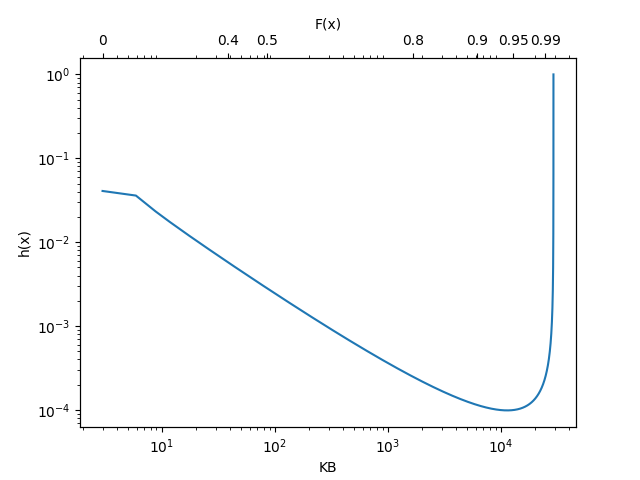
\includegraphics[width=0.99\textwidth]{Chapter3/Figures/hazard_pareto}
		\caption{Hazard function.}
		\label{fig:hazard}
	\end{subfigure}%
	\caption{WS workload}
\end{figure}%
Figure \ref{fig:opt-subth-lowpserver} shows the results. On the abscissa there are the cut percentile at which the load balance threshold truncate the job size distribution. The lower bound (blue curve) is the load balance threshold value, varying in order to cut the workload cdf at a given percentile.  The upper bound (black dashed line) is the length of the longest job in the workload. Finally, it is shown the optimal sub-threshold of the low priority server $s_2$ (orange line), computed for each imposed cut. The notable result is that starting from nearly the 90-th percentile, it is not convenient to use PQs on the low priority server for demotion. Indeed, the optimal sub-threshold saturates to the extreme of the support. This is coherent with the increasing hazard function at high percentiles. Indeed, it was discussed (\S \ref{sec:las}) that LAS scheduling is convenient when the hazard rate $h(x)$ is a decreasing function.\\
This experiment also explained why the performances are so bad when the dimensions of the system increase. Remember that subsequent servers observe cut workloads, whose heavy-tailed property is gradually destroyed. Thus, the heavy-tail of the DC-wide workload is progressively reduced as considering lower and lower priority servers. Under this condition, it is not recommended to schedule with LAS discipline, therefore intra-server demotion is a downside. Intuitively, since lower priority servers receive only jobs corresponding to high percentiles, long flows cause protracted starvation to each other, with the longest flows being the more penalized. \\
As a side note, if the variability becomes so low, it would be even recommended to serve jobs with FIFO and not PS. As a trivial example of low variability, suppose to schedule two flows $f_1, f_2$ both of size 10 (bits/bytes/packets,...). Denote as $T(f_i)$ the average flow completion time of flow $i$, expressed in transmission slots. FIFO scheduling would give:
\[
	T_{FIFO}(f_1) = T_{FIFO}(f_2) = \dfrac{10+20}{2} = 15
\]
Instead, PS scheduling would be worse:
\[
T_{PS}(f_1) = T_{PS}(f_2) = \dfrac{19+20}{2} = 19.5
\]
\subsubsection{Flow synchronization}
The second issue we have identified is flow synchronization. Consider the topology with $K$=5 and $N$=2. We plot the CDF of the flow inter-arrival time, that is the distribution of the time elapsed between two consecutive job arrivals. 
\begin{figure}
	\centering
	\captionsetup{width=.75\linewidth}
	\begin{subfigure}{.5\textwidth}
		\centering
		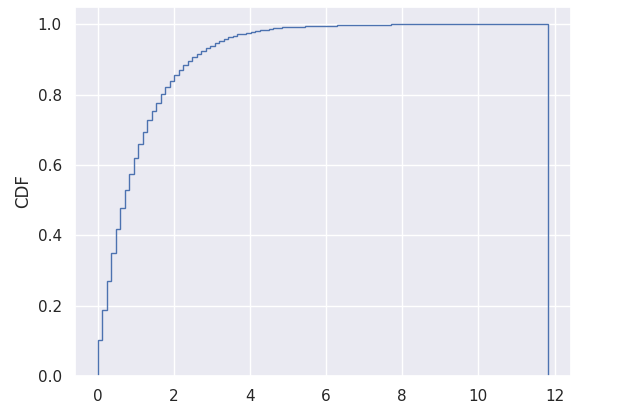
\includegraphics[width=0.99\textwidth]{Chapter3/Figures/inter_arrival0_PS}
		\caption{CDF at $s_1$}
		\label{fig:iatimes-ps-s1}
	\end{subfigure}%
	\hfill
	\begin{subfigure}{.5\textwidth}
		\centering
		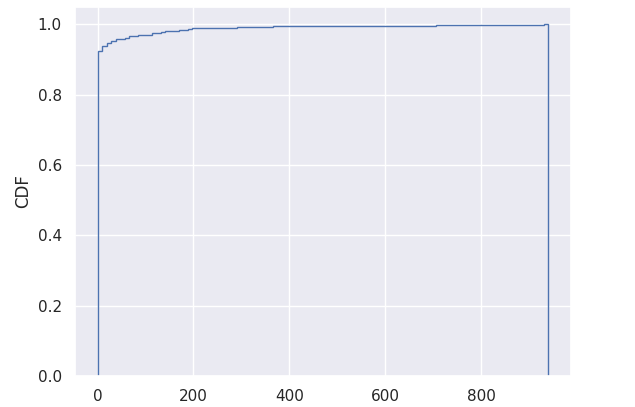
\includegraphics[width=0.99\textwidth]{Chapter3/Figures/inter_arrival4_PS}
		\caption{CDF at $s_5$}
		\label{fig:iatimes-ps-s5}
	\end{subfigure}%
	\caption{Flow synchronization with PS discipline. Flow inter-arrival distributions at highest and lowest priority servers.}
	\label{fig:iatimes-ps}
\end{figure}%
As usual the notation $s_i$ indicates the servers, from higher to lower priority. By looking at the distribution on the lowest priority server $s_5$, there is an anomalous spike at 0ms inter-arrival, that spans the y-axis up to the 90-th percentile (Fig.\ref{fig:iatimes-ps-s5}). This is strange because all flows enter the system from $s_1$, hence we expected a flatter cumulative function, at least at the beginning. Instead, its shape discloses bursts of flow arrivals, with many of them arriving synchronized at the same time instants. \\
We explain this synchronization as a joint result of processor sharing, strict priority and flow demotion. Consider a generic set of flows $\mathcal{F}$, whose sizes are such that the all flows end their service in $s_5$. Denote with $Q_i^j$ the $i$-th priority queue of the $j$-th server, with the usual order and notation followed in the theoretical model of spatial diversity (\S \ref{sec:complete-model}). Flow $\tilde{f}$ enters the system through $s_1$ and starts its service. Denote with $\mathcal{F}^\prime$  all flows $f \in \mathcal{F} \setminus \{\tilde{f}\}$ entered the system before $\tilde{f}$. Instead, use $\mathcal{F}^{\dprime}$ for all flows $f \in \mathcal{F} \setminus \{\tilde{f}\}$ arriving after $\tilde{f}$ but still while $\tilde{f}$ is served by the first server. Flows in $\mathcal{F}^{\dprime}$ either share the processor with $\tilde{f}$ in the high priority queue $Q_1^1$ or are served with higher priority of $\tilde{f}$ because this is already in the lowest priority queue $Q_2^1$.  In both cases, $\tilde{f}$ is the first to be shifted to the lowest PQ and at this point happens the synchronization. As a matter of fact $\tilde{f}$ doesn't leave the lowest PQ until all flows $f \in \mathcal{F}^{\dprime}$ do. First it waits them in $Q_2^1$ because of strict priority scheduling among PQs, then it shares the processor with them. When finally $\tilde{f}$ is rerouted to the subsequent server $s_2$, those flows in $\mathcal{F}^\prime$ that are yet served in $s_2$, again synchronize themselves with --- at least --- $\tilde{f}$.  In other words, the combination of spatial diversity, processor sharing and strict priority create on-off bottlenecks that lead to synchronization. This explanation is validated by the fact that in case of FIFO we do not observe any of this effect. Figure \ref{fig:iatimes-fifo} reports the inter-arrivals at the lowest priority servers $s_5$. Not surprisingly, for $s_1$ it is identical to the one obtained with PS.
\begin{figure}
	\centering
	\begin{subfigure}{.45\textwidth}
		\centering
			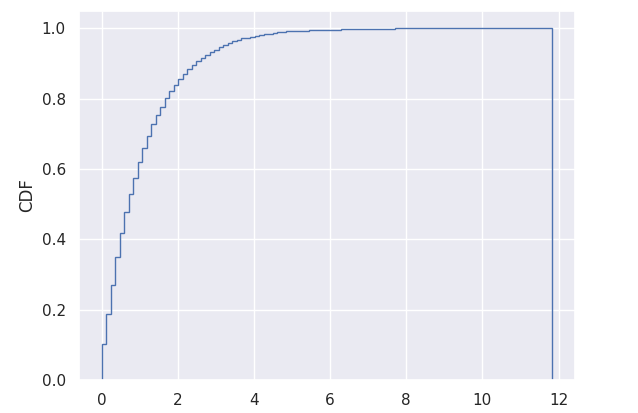
\includegraphics[width=0.99\textwidth]{Chapter3/Figures/inter_arrival0_FIFO}
		\caption{CDF at $s_1$}
		\label{fig:iatimes-fifo-s1}
	\end{subfigure}%
	\hfill
	\begin{subfigure}{.45\textwidth}
		\centering
		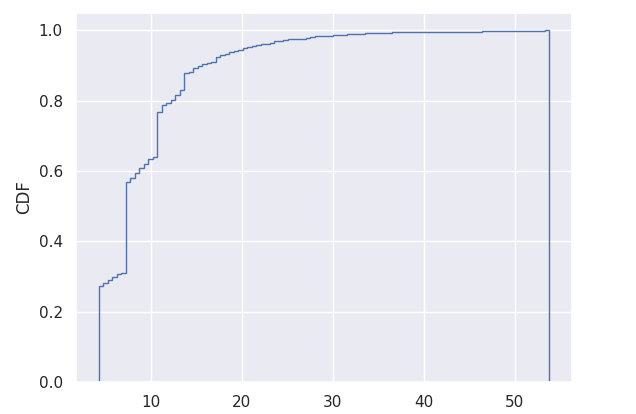
\includegraphics[width=0.99\textwidth]{Chapter3/Figures/inter_arrival4_FIFO}
		\caption{CDF at $s_5$}
		\label{fig:iatimes-fifo-s5}
	\end{subfigure}%
	\caption{FIFO does not suffer flow sync. CDF of inter-arrivals shown only for $s_5$}
	\label{fig:iatimes-fifo}
\end{figure}%

We think that this flow synchronization arises also in the system without spatial diversity and it is something not highlighted by authors of PIAS. Instead of showing at server level, we think that bursts arrivals could occur at priority queue level, especially when $N$ is large. However, since lower priority queues are served in strict priority only when high PQs are empty, we guess that these bursts are also less penalizing. \textcolor{red}{QUAL'ERA IL COMMENTO DI ANDREA ? CHE IN UNA RETE A PACCHETTO PROBABILMENTE NON SI VEDE COSI TANTO?? PERCHE' ? PERCHE' IL FLUSSO NON CE L'HAI TUTTO SUBITO MA LE TCP SOURCES TE LO MANDANO SEGMENTATO?}
\subsection{Final comparison}
\label{sec:final-comparison}
In previous sections were undisclosed the effects of spatial diversity under different settings, in order to understand which is the best dimensioning of the system in terms of number of servers and priority queues. At the same time were highlighted two implications of spatial diversity on the performance of strict priority scheme with demotion. In this section we want to exploit the insights just gained and compare SD-MLFQ with the system without spatial diversity and ES-N threshold assignment. Ultimately, showing that the system with spatial diversity outperforms the other would be our final goal. As usual, we evaluated both FIFO and PS discipline and we show results for the Web search workload only. Whenever load balance thresholds are optimized, we labeled the algorithm as SD-MLFQ-OPT. Results with FIFO are coherent with previous analysis. \\
First, the benefits of spatial diversity on a FIFO system with MLFQ demotion are more remarked for increased dimensionality. Either an increase in the number of servers (Fig. \ref{fig:esn-vs-sdmlfq-fifo-fixed-N}) or an increase in the number of priorities (Fig. \ref{fig:esn-vs-sdmlfq-fifo-fixed-K}), offer to short flows a chance to get rid earlier of their wait behind long flows. Additionally, FIFO does not suffer flow synchronization problem. For similar reasons SD-MLFQ achieves better performances in respect to ES-N for all considered combination of $K$ and $N$, making spatial diversity a very attractive solution for systems where FIFO at job level is a hard constraint.
\begin{figure}
	\centering
	\captionsetup{width=.8\linewidth}
	\begin{subfigure}{.5\textwidth}
		\centering
		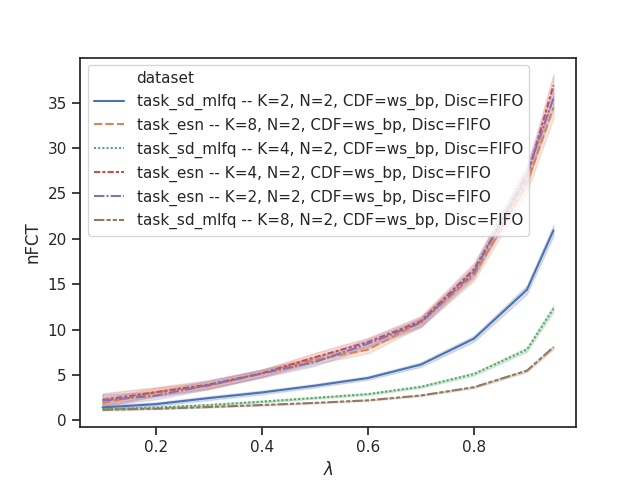
\includegraphics[width=0.99\textwidth]{Chapter3/Figures/comparison_esn_vs_mlfq_fifo_vs_servers}
		\caption{Fixed $N$=2 priorities per server}
		\label{fig:esn-vs-sdmlfq-fifo-fixed-N}
	\end{subfigure}%
	\hfill
	\begin{subfigure}{.5\textwidth}
		\centering
		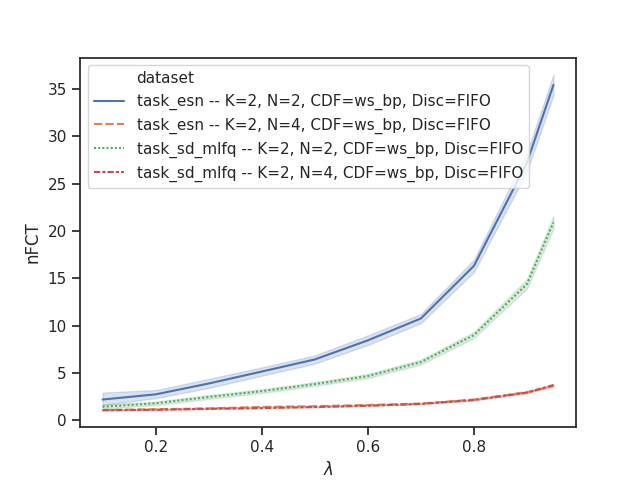
\includegraphics[width=0.99\textwidth]{Chapter3/Figures/comparison_esn_vs_mlfq_fifo}
		\caption{Fixed $K$=2 parallel servers}
		\label{fig:esn-vs-sdmlfq-fifo-fixed-K}
	\end{subfigure}%
	\caption{Comparison among SD-MLFQ and ES-N for web search workload and FIFO. Results plotted with 99\% confidence interval.}
\end{figure}%
On the contrary, the Processor Sharing discipline is less compatible with spatial diversity. Figure \ref{fig:esn-vs-sdmlfq-ps-fixed-N} depicts the comparison between SD-MLFQ and ES-N for fixed values of $N$ and variable $K$. In particular, only $N$=1 and $N$=2 have been considered because we have seen that with many priority queues per server and spatial diversity we incur in some impairments (\S \ref{sec:sd-impairments}). Nonetheless, results for fixed $K$ and varying $N$ at $\lambda = 0.9$ can be found in the summarizing Table \ref{tab:esn-vs-sdmlfq} and are coherent with our intuitions. The principal insights can be grasped from Figures \ref{fig:esn-vs-sdmlfq-ps-fixed-N-2}-Fig. \ref{fig:esn-vs-sdmlfq-ps-fixed-N-1}.  Unfortunately it is clear SD-MLFQ becomes rapidly worse than ES-N when $N \times K$ grows. Even for small dimensioning, such as $K \times N = 4$, ES-N is slightly better than SD-MLFQ.
\begin{figure}[!tb]
	\centering
%	\captionsetup{width=.8\linewidth}
	\begin{subfigure}{.5\textwidth}								   
		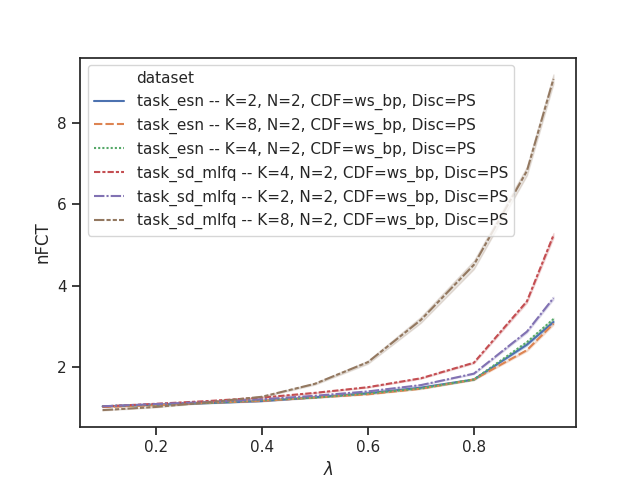
\includegraphics[width=0.99\textwidth]{Chapter3/Figures/comparison_esn_vs_mlfq_ps_vs_servers}
		\caption{$N$=2}	
		\label{fig:esn-vs-sdmlfq-ps-fixed-N-2}
	\end{subfigure}%
	\hfill
	\begin{subfigure}{.5\textwidth}			
		\centering
		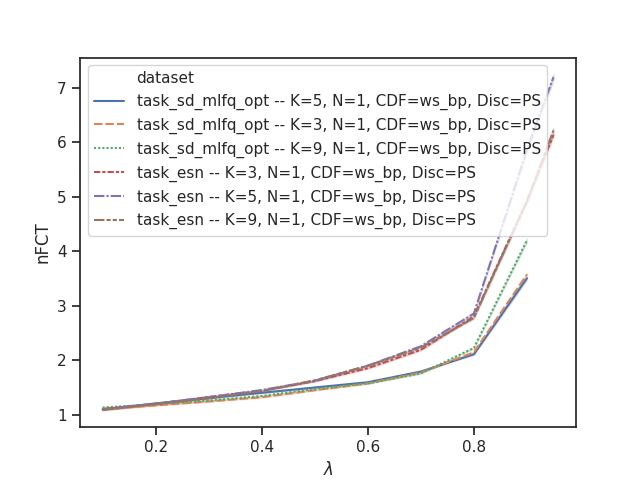
\includegraphics[width=0.99\textwidth]{Chapter3/Figures/comparison_esn_vs_mlfq_ps_n11}
		\caption{$N$=1}
		\label{fig:esn-vs-sdmlfq-ps-fixed-N-1}
	\end{subfigure}%
	\caption{Comparison among SD-MLFQ and ES-N for web search workload and PS at 99\% confidence interval. For both figures the number of priorities $N$ is fixed.}	
	\label{fig:esn-vs-sdmlfq-ps-fixed-N}
\end{figure}%
In the summarizing table is also present the detailed comparison for all considered scenarios both with optimized and proportionate split thresholds. The optimized load balance thresholds are very effective for the system without intra-server demotion, that is with a single queue. This comes at no surprise since in such a condition our intelligent load balancing is the only way to separate short and long flows. Indeed, for $N$=1 the SD-MLFQ-OPT wins also over ES-N (Fig.\ref{fig:esn-vs-sdmlfq-ps-fixed-N-1}), which randomly load balance flows on available servers, thus mixing flows of any size. The effect of optimal load balancing start to be less prevalent than the effect of priority queues for $N \ne 1$. When $N$=4 SD-MLFQ-OPT achieves worse performances than SD-MLFQ. 
\begin{table}[]
	\centering
	\begin{tabular}{lllll}
		\hline
		\multicolumn{2}{l}{{\color[HTML]{000000} Scenario}} &
		{\color[HTML]{000000} ES-N} &
		{\color[HTML]{000000} SD-MLFQ-OPT} &
		{\color[HTML]{000000} SD-MLFQ} \\ \hline
		{\color[HTML]{000000} } &
		{\color[HTML]{000000} K=3} &
		{\color[HTML]{000000} 9.12} &
		{\color[HTML]{000000} 6.61} &
		{\color[HTML]{000000} 9.59} \\
		{\color[HTML]{000000} } &
		{\color[HTML]{000000} K=5} &
		{\color[HTML]{000000} 9.37} &
		{\color[HTML]{000000} 6.36} &
		{\color[HTML]{000000} 9.71} \\
		\multirow{-3}{*}{{\color[HTML]{000000} N=1}} &
		{\color[HTML]{000000} K=9} &
		{\color[HTML]{000000} 8.77} &
		{\color[HTML]{000000} 8.26} &
		{\color[HTML]{000000} 10.12} \\ \hline
		{\color[HTML]{000000} } &
		{\color[HTML]{000000} K=3} &
		{\color[HTML]{000000} 4.20} &
		{\color[HTML]{000000} 4.62} &
		{\color[HTML]{000000} 5.52} \\
		{\color[HTML]{000000} } &
		{\color[HTML]{000000} K=5} &
		{\color[HTML]{000000} 4.32} &
		{\color[HTML]{000000} 7.67} &
		{\color[HTML]{000000} 7.95} \\
		\multirow{-3}{*}{{\color[HTML]{000000} N=2}} &
		{\color[HTML]{000000} K=9} &
		{\color[HTML]{000000} 4.08} &
		{\color[HTML]{000000} 13.41} &
		{\color[HTML]{000000} 14.59} \\ \hline
		{\color[HTML]{000000} } &
		{\color[HTML]{000000} K=3} &
		{\color[HTML]{000000} 2.64} &
		{\color[HTML]{000000} 4.87} &
		{\color[HTML]{000000} 5.34} \\
		{\color[HTML]{000000} } &
		{\color[HTML]{000000} K=5} &
		{\color[HTML]{000000} 2.70} &
		{\color[HTML]{000000} 14.76} &
		{\color[HTML]{000000} 13.09} \\
		\multirow{-3}{*}{{\color[HTML]{000000} N=4}} &
		{\color[HTML]{000000} K=9} &
		{\color[HTML]{000000} 2.57} &
		{\color[HTML]{000000} 13.29} &
		{\color[HTML]{000000} 11.56} \\ \cline{1-5} 
	\end{tabular}
	\caption{Summary of the comparison for PS discipline and $\lambda$=0.9}
	\label{tab:esn-vs-sdmlfq}
\end{table}

